\section{Описание и разработка распределенной системы доступа к базам данных на основе программных агентов платформы JADE}
\subsection{Краткое описание разрабатываемой системы}
Описываемая распределенная система разрабатывалась на объектно-ориентированном языке программирования Java. Ядром системы является программная платформа JADE, включающая в себя как набор классов для реализации агентно-ориентированных приложений, так и инструментарий для запуска, управления и настройки платформ, контейнеров и агентов.

	Для хранения данных используется свободная объектно-ориентированная система управления базами данных Postgresql. В качестве библиотеки с базой используется jdbc-драйвер. Взаимодействие системы с пользователем осуществляется с помощью стандартного графического оконного интерфейса на основе средств, представляемых библиотекой Swing.

	Управление процессом разработки осуществляется с помощью системы контроля версий GIT. Это позволяет контролировать все изменения в проекте, фиксировать контрольные точки и этапы разработки, а также мгновенно переключаться между ними. Исходный код проекта синхронизируется с сервером github.com. Это позволяет иметь доступ к проекту из любого места, где есть доступ к сети интернет.

	Сборка проекта, поиск и установка зависимостей осущестляется с помощью фреймворка Maven. Это позволяет в значительной мере сократить сроки и усилия по развертыванию, переносу, изменению конфигурации проекта и другим подобным операциям.

В качестве операционной системы используется дистрибутив свободной операционной системы Linux~--- Ubuntu 12.04 LTS. Ubuntu пригодна для решения как настольных, так и серверных задач. Система включает в себя более 16 тысяч программных пакетов. Ubuntu перекрывает потребность во всех разновидностях настольного программного обеспечения от редактирования текстов и электронных таблиц до поддержки веб-серверов и программирования. 

Средой разработки служит бесплатная реализация одной из наиболее мощных IDE для разработки приложений на Java~--- Intellij IDEA Community Edition. Среди ее основных возможностей следует выделить следующее:
\begin{itemize}
\item <<умное>> автодополнение, инструменты для анализа качества кода, удобная навигация, расширенные рефакторинги и форматирование для Java, Groovy, Scala, Clojure и Erlang;
\item профессиональный набор инструментов для разработки Android-приложений;
\item поддержка JavaFX 2.0, интеграция с SceneBuilder;
\item дизайнер интерфейса для Swing;
\item интеграция с автоматизированными инструментами сборки и управления проектом, включа Maven, Gradle, Ant и другими;
\item инструменты для тестирования с поддержкой JUnit, TestNG, Spock, ScalaTest и spec2;
\item интеграция с системами управления версиями, включая Git, Subversion, Mercurial и CSV.
\end{itemize}

	Проектируемая распределенная система будет состоять из наборов взаимодействующих между собой программных агентов, часть из которых будет находиться на локальном контейнере платформы и обрабатывать пользовательские  запросы к базе, а часть~--- на удаленных контейнерах, имеющих в своем составе сервер базы данных, отвечая за обработку запросов от локальных агентов-клиентов, передачу этих запросов в СУБД, обработку и передачу ответа. Пользователь, взаимодействуя с графическим интерфейсом, будет формировать запросы, отправляемые первоначально на агент-контроллер, отвечающий за логику  межагентного взаимодействия, и получать ответы от удаленных серверов в главном окне программы.

\begin{figure}[h!]
\center{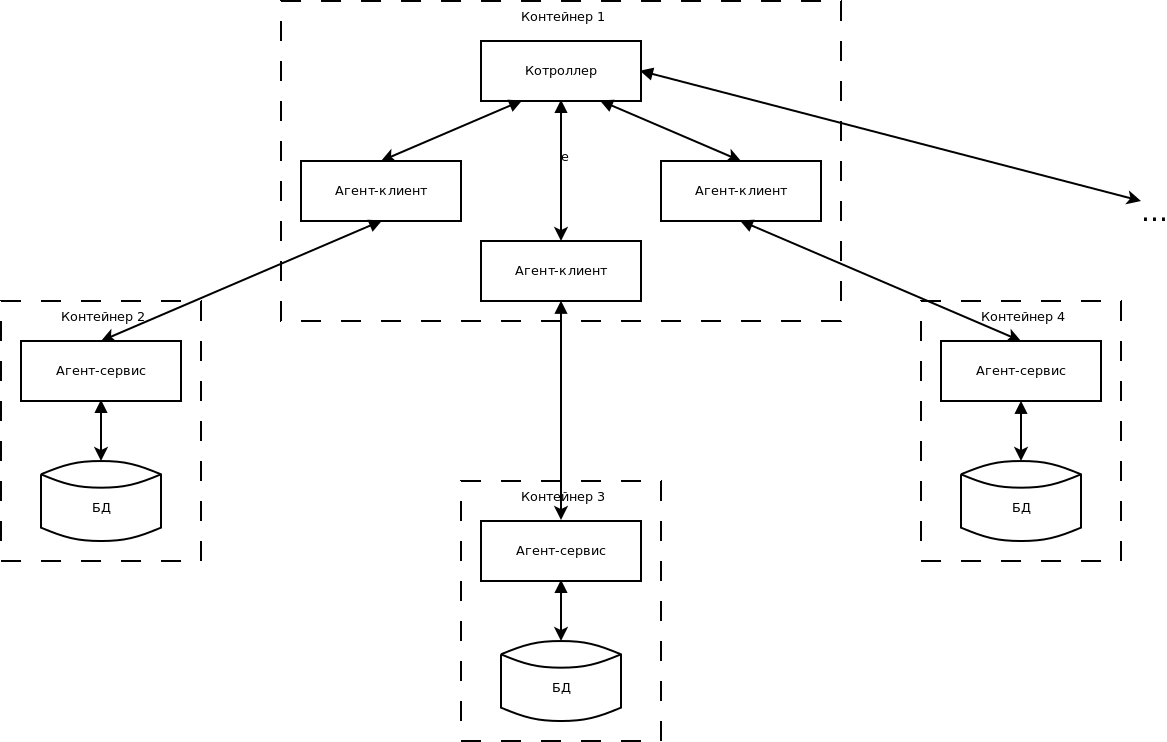
\includegraphics[width=0.9\linewidth]{common-scheme}}
\caption{Общая структура разрабатываемого приложения}
\label{3:common-scheme}
\end{figure}

Кроме этого, следует отметить, что изначально система запускается на локальном контейнере, а затем с помощью технологии мобильных агентов перемещает агенты-сервисы на имеющиеся в составе платформы удаленные контейнеры. Это позволяет иметь полную независимость от конфигураций серверных машин, версий и взаимной совместимости сервисной части системы на каждом удаленном узле. Более того, не потребуется помощь технического специалиста по настройке системы на каждом узле, не потребуется помощь и при масштабировании системы. Приложению достаточно увидеть новый контейнер в составе системы (ествественно, имеющей в своем составе необходимые для функционирования системы зависимости: JADE-платформа, без которой в общем-то и невозможно взаимное обнаружение и взаимодействие контейнеров внутри платформы, СУБД postgresql и т.д.), после чего, по указанию пользователя, будет произведена загрузка агента-сервиса на удаленный контейнер и его дальнейшее функционирование в рамках распределенной системы.

	На рисунке~\ref{3:seq-launch} приведена диаграмма последовательности запуска приложения и добавления нового узла (контейнера) в состав распределенной системы. Подобная последовательность событий и действий является аналогичной (начиная с события регистрации нового контейнера) при добавлении новых узлов в состав системы.

\begin{figure}[h!]
\center{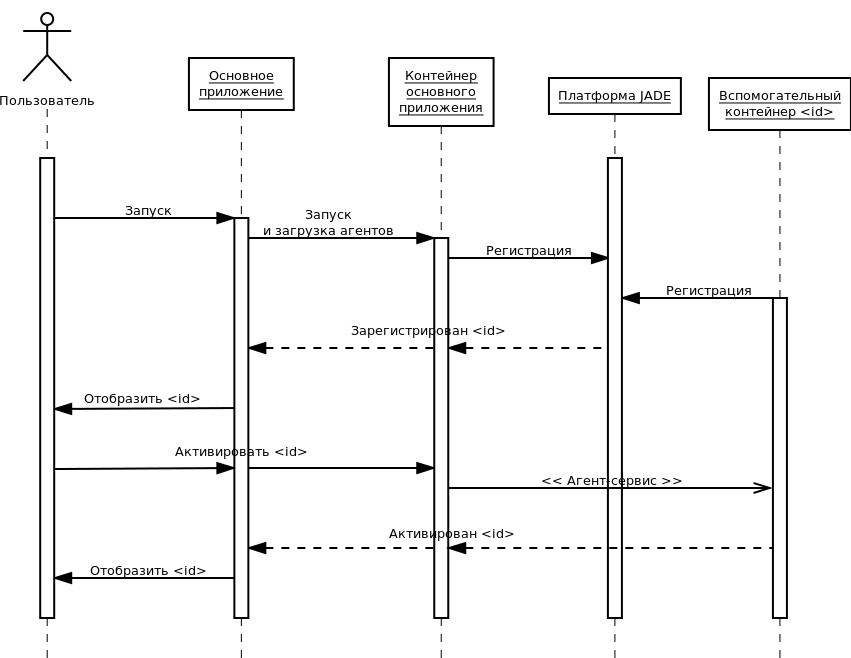
\includegraphics[width=0.9\linewidth]{seq-launch}}
\caption{Диаграмма последовательности запуска приложения и добавления нового узла}
\label{3:seq-launch}
\end{figure}

После загрузки агента-сервиса на удаленный контейнер происходит уведомление агента-контроллера, расположенного в составе модуля управления и  межагентного взаимодействия, после чего для агента-сервиса создается агент-клиент, который впоследствии будет уже напрямую обращаться к данному сервису.

Выбирая активные платформы, пользователь может обмениваться с ними информацией, не заботясь об их конфигурациях и местоположении.

Из доступных операций пользователю предоставляется возможность:
\begin{itemize}
\item получать список таблиц, расположенных на удаленном контейнере;
\item отображать контент выбранной таблицы контейнера;
\item редактировать данные выбранной таблицы;
\item добавлять данные в выбранную таблицу;
\item добавлять данные в выбранную таблицу с автоматическим реплицированием на активные контейнеры при наличии на них этой же таблицы;
\item выполнять RAWSQL-запросы на выбранный контейнер;
\item выполнять RAWSQL-запросы на все активные контейнеры.
\end{itemize}

\subsection{Описание состава пакетов системы}
Проект распеределенной системы разрабатывался в интегрированной среде разработки Intellij IDEA Community Edition. На левой панели расположены классы и интерфейсы проекта. На средней панели расплоложены вкладки настроек проекта. Справа располагаются поля настроек конкретной вкладки.
\begin{figure}[h!]
\center{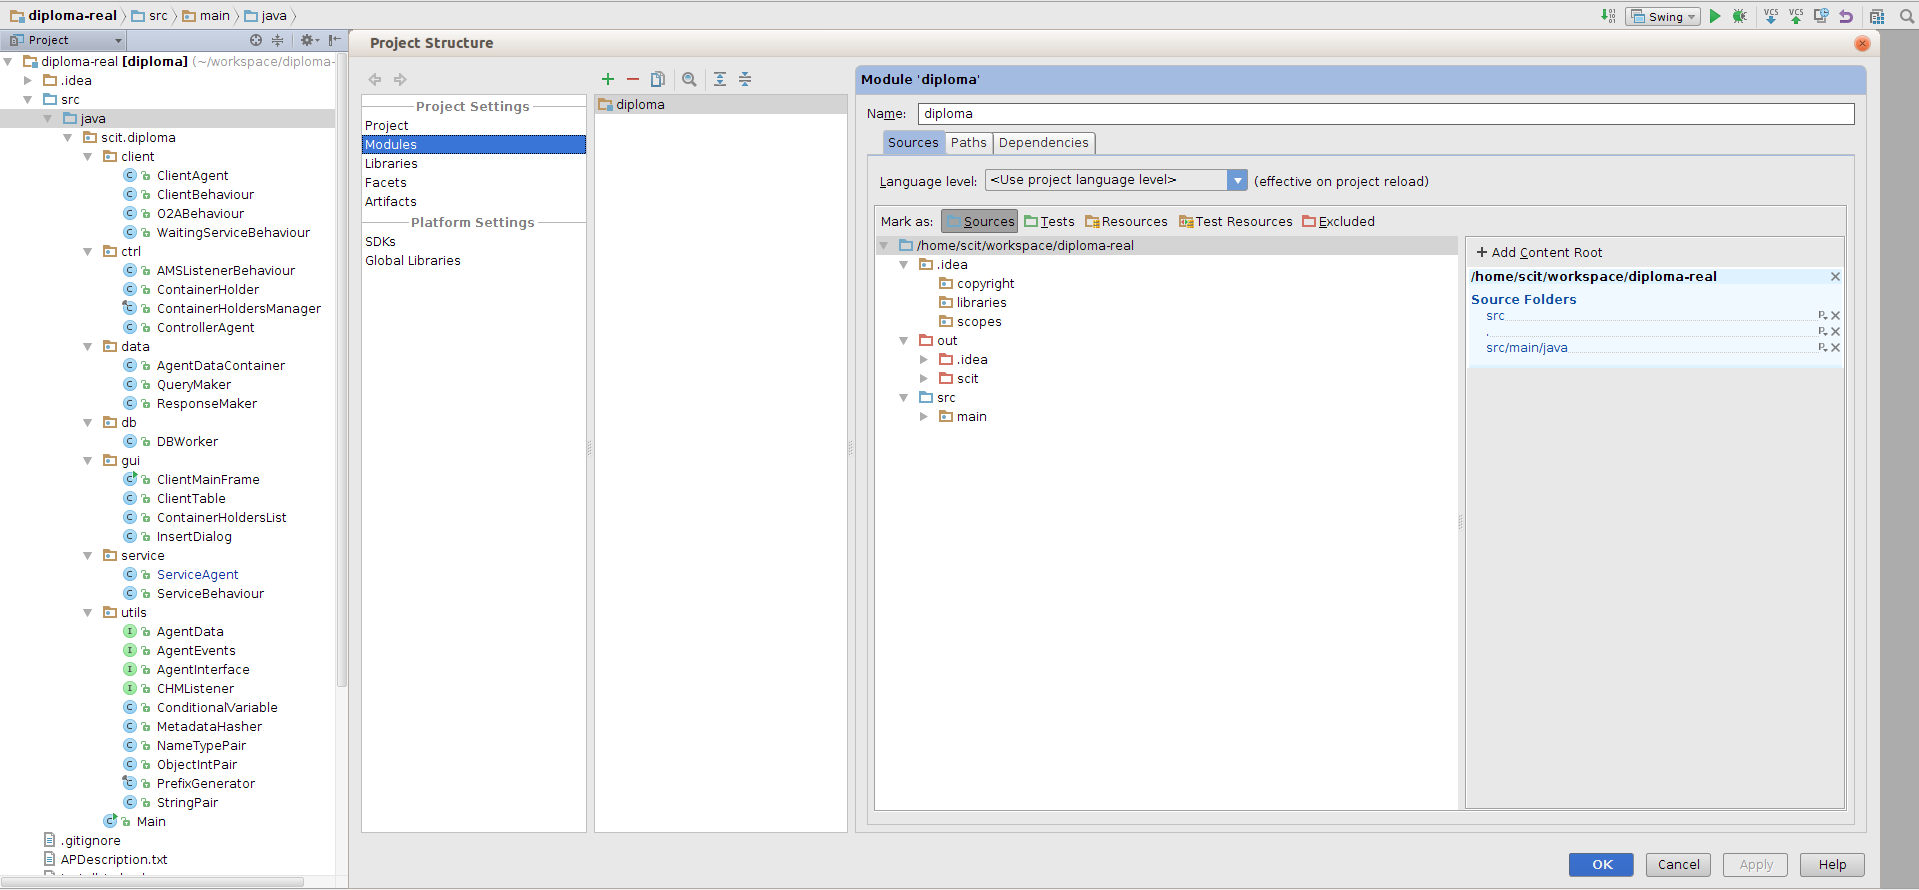
\includegraphics[width=1\linewidth]{ide}}
\caption{Состав проекта в интегрированной среде разработки Intellij IDEA}
\label{3:ide}
\end{figure}
Рассмотрим структуру, состав и назначение имеющихся классов и интерфейсов распределенной системы, сгруппированных в отдельные логические пакеты.

\subsubsection{Состав пакета client}
Данный пакет содержит классы, входящие в состав агента-клиента. Основной класс ClientAgent, как видно из названия, реализует логику работы самого агента.

\paragraph{Класс ClientAgent}
Класс агента, как правило реализует основной метод setup(), в котором происходит инициализация агента, добавление поведений и другие операции, связанные с функционированием агента.
Ниже показано содержимое метода setup() класса ClientAgent:
\begin{lstlisting}
protected void setup() {
    setEnabledO2ACommunication(true, 0);
    Object[] args = getArguments();

    switch(args.length) {
        case 3:
            serviceAID = (AID) args[2];
        case 2:
            agentInterface = (AgentInterface) args[1];
        case 1:
            ConditionalVariable startUpLatch = (ConditionalVariable) args[0];
            startUpLatch.signal();
    }

    ((AgentEvents) agentInterface).onEvent(new AID(getName(), AID.ISLOCALNAME), AgentEvents.EVENT_CLIENT_READY);
    addBehaviour(new O2ABehaviour());
}
\end{lstlisting}
По-сути, содержимое метода отвечает за настройку приема данных от внешних классов, не являющихся агентами. Это реализовано с помощью технологии Object2Agent communication. Для этого необходимо включить поддержку взаимодействия O2A методом setEnabledO2ACommunication().

Далее, в контрукции switch() происходит выборка доступных аргументов, с которыми был запущен агент.

Первым аргументом (порядок аргументов идет с конца) передается мьютекс ConditionalVariable, который позволяет внешнему окружению дождаться запуска и инициализации агента. В противном случае, данные агентом получены не будут.

Второй аргумент хранит подписчика на события агента. Интерфейс AgentInterface имеет два интерфейса-потомка: AgentData и AgentEvents. Первый из них отвечает за уведомление о поступающих от агента данных, а второй~--- о возникающих событиях. В данном случае, агент посылает событие EVENT\_CLIENT\_READY, означающее готовность агента к функционированию.

Третий аргумент хранит AID~--- идентификатор~--- агента-сервиса, за которым <<закреплен>> данный агент-клиент.

В конце метода происходит добавление поведения O2ABehaviour, которое обрабатывает входящие данные от внешних модулей приложения.

\paragraph{Класс ClientBehaviour}
\begin{figure}[h!]
\center{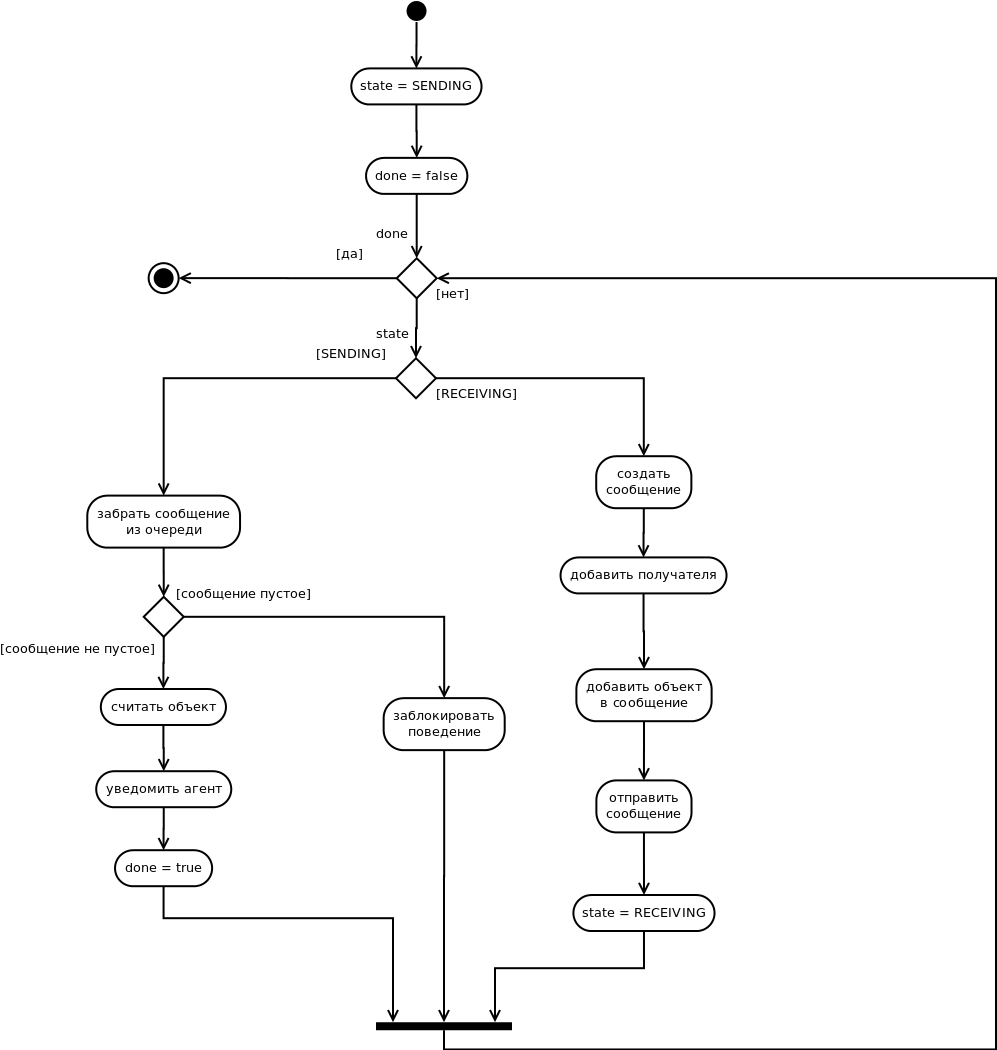
\includegraphics[width=1\linewidth]{client-beh}}
\caption{Диаграмма деятельности поведения ClientBehaviour}
\label{3:client-beh}
\end{figure}
Основным методом объектов класса Behaviour является метод action(). Данный метод вызывается платформой по правилам, заложенным в реализации класса.

\begin{lstlisting}
public void action() {
    ACLMessage message = null;

    switch (state) {
        case SENDING:
            message = new ACLMessage(ACLMessage.REQUEST);
            message.addReceiver(aid);

            try {
                message.setContentObject(agentDataContainer);
            } catch (IOException e) {
                e.printStackTrace();
            }

            myAgent.send(message);
            state++;
            break;
        case RECEIVING:
            message = myAgent.receive();
            if(message != null) {
                try {
                    agentDataContainer = (AgentDataContainer) message.getContentObject();
                } catch (UnreadableException e) {
                    e.printStackTrace();
                }

                AgentData agentData = (AgentData) ((ClientAgent) myAgent).getAgentInterface();
                AID aid = new AID(myAgent.getName(), AID.ISLOCALNAME);
                agentData.onData(aid, agentDataContainer);
                done = true;
            } else {
                block();
            }

            break;
    }
}
\end{lstlisting}
Функционирование основного поведения агента-клиента реализовано в виде <<машины состояний>>. На первом этапе поведение функционирует в состоянии отправки запроса агенту сервиса, для чего формируется соотвестствующее ACL сообщение. На втором~--- в ожидании ответа от сервиса. В конце выполнения поведения происходит уведомление агента о полученных данных от агента-сервиса.
На рисунке~\ref{3:client-beh} представлена диаграмма деятельности данного класса.

\paragraph{Класс O2ABehaviour}
Класс O2ABehaviour содержит циклический опрос очереди O2A-сообщений. При отсутствии сообщений поведение блокируется методом block() до появления нового сообщения в очереди.
\begin{lstlisting}
public void action() {
    AgentDataContainer agentDataContainer = (AgentDataContainer) myAgent.getO2AObject();
    if(agentDataContainer != null) {
        myAgent.addBehaviour(new ClientBehaviour(myAgent, agentDataContainer));
    } else {
        block();
    }
}
\end{lstlisting}

\subsubsection{Состав пакета service}
\paragraph{Класс ServiceAgent}
Основной класс пакета service~--- ServiceAgent. Его метод setup() аналогичен содержимому метода класса ClientAgent. Помимо этого, класс ServiceAgent реализует методы beforeMove() и afterMove()~--- это callback-методы, вызываемые платформой JADE, соотвественно до и после операции перемещения агента. Метод beforeMove() не содержит функциональной логики, а служит лишь для печати отладочной информации на консоль. Метод afterMove() добавляет новое поведение в состав агента, и посылает сообщение агенту-контроллеру о своем перемещении.
\begin{lstlisting}
protected void afterMove() {
    addBehaviour(new ServiceBehaviour(this));

    System.out.println("After move: " + here());
    ACLMessage msg = new ACLMessage(ACLMessage.INFORM);
    msg.setConversationId(ControllerAgent.CONTROLLER_AGENT_CONVERSATION_ID);
    AID dest = new AID(ContainerHoldersManager.CONTROLLER_AGENT_NAME, AID.ISLOCALNAME);
    msg.setContent(getName());
    try {
        msg.setContentObject(here());
    } catch (IOException e) {
        e.printStackTrace();
    }
    msg.addReceiver(dest);
    send(msg);
}
\end{lstlisting}

\paragraph{Класс ServiceBehaviour}
\begin{figure}[h!]
\center{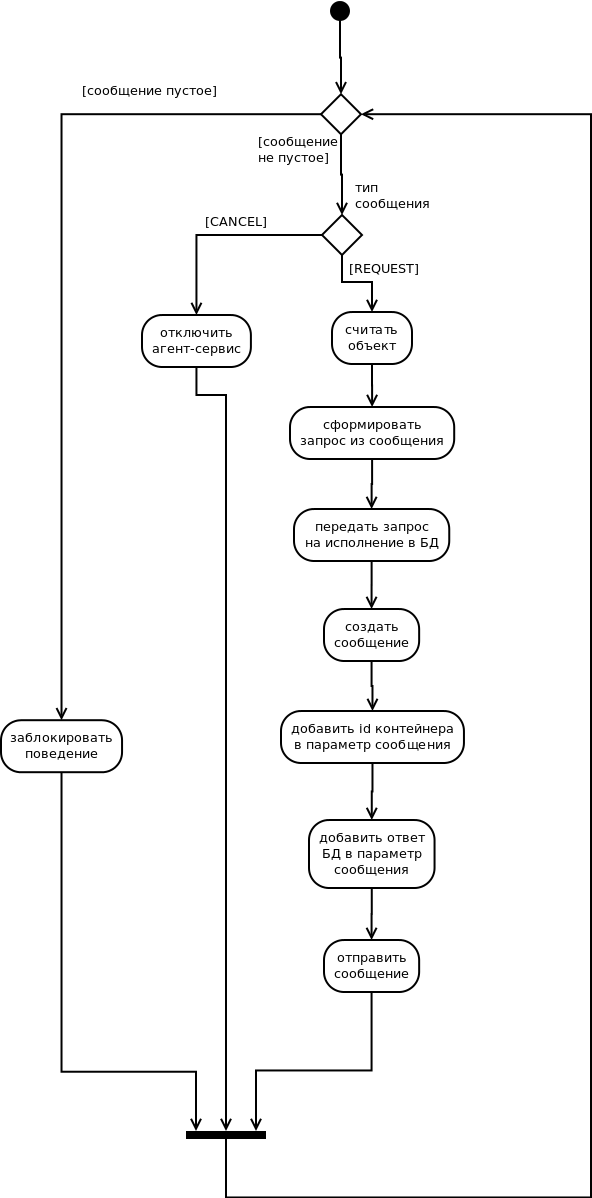
\includegraphics[width=0.6\linewidth]{service-beh}}
\caption{Диаграмма деятельности поведения ServiceBehaviour}
\label{3:service-beh}
\end{figure}

Поведение агента-сервиса ServiceBehaviour содержит интерфейсы взаимодействия с базой данных узла посредством классов, предоставляемых пакетом db. Логически поведение разбито на две части: это обработка запроса с передачей его к СУБД и формирование и отправка ответа агенту-клиенту. Кроме этого, при получении сообщения с типом CANCEL сервис завершает свою работу.
\begin{lstlisting}
public void action() {
    ACLMessage msg = myAgent.receive();
    if (msg != null) {
        switch (msg.getPerformative()) {
            case ACLMessage.REQUEST:
                ACLMessage reply = msg.createReply();
                reply.setPerformative(ACLMessage.INFORM);
                AgentDataContainer agentDataContainer = null;

                try {
                    agentDataContainer = (AgentDataContainer) msg.getContentObject();
                    System.out.print(agentDataContainer);
                } catch (UnreadableException e) {
                    e.printStackTrace();
                }

                agentDataContainer = dbw.execute(agentDataContainer);
                agentDataContainer.setParam(AgentDataContainer.KEY_CONTAINER_NAME, myAgent.here().getName());

                try {
                    reply.setContentObject(agentDataContainer);
                } catch (IOException e) {
                    e.printStackTrace();
                }

                myAgent.send(reply);
                break;
            case ACLMessage.CANCEL:
                myAgent.doDelete();
                break;
        }
    } else {
        block();
    }
}
\end{lstlisting}
На рисунке \ref{3:service-beh} представлена диаграмма деятельности данного класса.

\subsubsection{Состав пакета ctrl}
Пакет ctrl включает в себя классы, осуществляющие организацию межагентного взаимодействия, управление контейнерами, входящими в состав платформы, уведомление внешних внеагентных компонентов о событиях внутри платформы.
\paragraph{Класс ControllerAgent}
Запускает поведение мониторинка контейнеров платформы.

Уведомляет основной программный контроллер ContainerHolderManager о процедуре перемещения агентов-сервисов.

\paragraph{Класс AMSListenerBahaviour}
Данное поведение регистрирует обработчик в плтаформе JADE. Внутри обработчика добавления новых контейнеров просходит получение идентификатора контейнера и передача его контроллеру приложения.
\begin{lstlisting}
public class AMSListenerBehaviour extends AMSSubscriber {
    public void installHandlers(Map handlersTable) {
        handlersTable.put(AddedContainer.NAME, new AddedContainerHandler());
    }

    public final class AddedContainerHandler implements EventHandler {
        public void handle(Event ev) {
            AddedContainer event = (AddedContainer) ev;
            ContainerID addedContainer = event.getContainer();

            ContainerHoldersManager.onContainerAdded(addedContainer);
        }
    }
}
\end{lstlisting}

\paragraph{Класс ContainerHolder}
Данный класс хранит всю информацию, относящующся к конкретному контейнеру, а также предоставляет все интерфейсы для взаимодействия агентов клиента и сервиса внешним компонентам приложения. Основые поля класса:

\begin{itemize}
\item AgentController client~--- агент-клиент, относящийся к данному контейнеру;
\item AID serviceID~--- идентификатор сервиса, который расположен на данному конейнеру;
\item ContainerID containerID~--- идентификатор контейнера;
\item isActive~--- флаг активности контейнера~--- активный контейнер имеет в своем составе запущенные агенты сервиса и клиента, относящиеся к данному контейнеру.
\end{itemize}

\begin{itemize}
\item doActivate()~--- активирует данный контейнер;
\item doExecute()~--- отправляет запрос на сервис. В качестве параметра передается объект класса AgentDataContainer;
\item onData()~--- callback-функция получения информации от сервиса;
\item onEvent()~--- callback-функция получения событий от сервиса.
\end{itemize}

\paragraph{Класс ContainerHoldersManager}
Класс ContainerHoldersManager служит для организации системы распределенных узлов. В нем хранится список доступных на платфрме контейнеров, а также создает системный контейнер и запускает агента-контроллера. Помимо этого, он занимается обработкой событий, поступающих от объектов класса ContainerHolder и, в свою очередь, делегирует эти события собственным подписчикам (listeners).

\subsubsection{Пакет db}
Данный пакет состоит лишь из одного класса: DBWorker, который отвечает за всю логику взаимодействия с базами данных. Основным методом данного класса является метод execute(), который, как видно из названия выполняет запрос к базе и обрабатывает полученный ответ для выдачи результата запрашиваемому агенту-сервису.
\begin{lstlisting}
public AgentDataContainer execute(AgentDataContainer agentDataContainer) {
    ...
    String dataType = AgentDataContainer.VALUE_DATA_TYPE_TABLES;

    connection = DriverManager.getConnection(url, user, password);

    if (agentDataContainer.getParam(KEY_REQUEST_STRING).equals(GET_TABLES_LIST)) {
        resultSet = connection.getMetaData().getTables(null, "public", "%", new String[]{"TABLE"});
    } else if (agentDataContainer.getDataLength() > 0) {
        boolean verified = verify(connection, agentDataContainer);
        if(verified) {
            dataType = AgentDataContainer.VALUE_DATA_TYPE_EMPTY;
            pst = connection.prepareStatement(agentDataContainer.getParam(KEY_REQUEST_STRING));

            Object[] dataRow = agentDataContainer.getData().get(0);
            for (int i = 0; i < agentDataContainer.getDataWidth(); i++) {
                pst.setObject(i + 1, dataRow[i], agentDataContainer.getMetadata()[i].getType());
            }

            pst.executeUpdate();
        }

        resultSet = null;
    } else {
        dataType = AgentDataContainer.VALUE_DATA_TYPE_CONTENT;
        pst = connection.prepareStatement(agentDataContainer.getParam(KEY_REQUEST_STRING));

        resultSet = pst.executeQuery();
    }

    outputAgentDataContainer = ResponseMaker.makeResponse(resultSet, agentDataContainer);
    outputAgentDataContainer.setParam(KEY_DATA_TYPE, dataType);
    ...
    return agentDataContainer;
}
\end{lstlisting}
В ветвлении if происходит определение типа входящего запроса:
\begin{itemize}
\item получение списка таблиц;
\item операция модификации/добавления данных в таблице;
\item операция получения данных из таблицы / RAW-SQL запрос.
\end{itemize}
Кроме того, в этом методе происходит верификация корректности запроса при обращении к таблицам: это необходимо для операций репликации на всех активных узлах.

Соединение создается в строке connection = DriverManager.getConnection(). Класс DriverManager заведует драйверами, соединениями, а также трассировкой. В данном случае вызывается статический метод getConnection(). Этот метод просматривает список драйверов и, если находит подходящий к указанному URL, то создает и возвращает соединение. В противном случае выбрасывает исключение с текстом: "No suitable driver found". В качестве аргументов данный метод принимает URL к базе, имя и пароль пользователя.

Запрос для исполнения формирутеся с помощью метода prepareStatement() класса Connection. Запрос может состоять как из одной лишь текстовой строки, так и содержать объекты-параметры. Первая задается непостредственно в аргуенте метода, а последние~--- добавляться в запрос методов setObject(). Исполнение производится методом executeQuery(), либо executeUpdate() для выполнения операций вставки и модификаций в базе.

Ниже представлена архитектура JDBC, в рамках которой взаимодействует и базой данный, в том числе, и данное приложение, используя JDBC server.
\begin{figure}[h]
\center{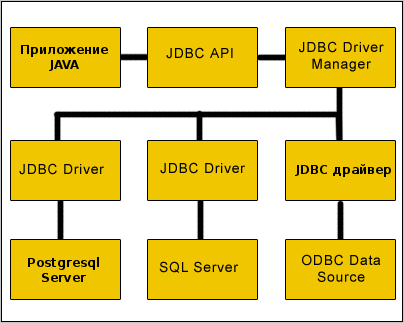
\includegraphics[width=0.7\linewidth]{jdbc}}
\caption{Взаимодействие Java-проложения с сервером БД}
\label{3:jdbc}
\end{figure}

\subsubsection{Пакет data}
\paragraph{Класс AgentDataContainer}
Данный класс является одним из наиболее универсальным и используемых сущностей в архитектуре приложения. Он пронизвыает буквально все уровни распределенной системы: начиная от классов графического пользовательского интерфейса, заканчивая обработчиком взаимодействия с сервером базы данных на удаленном узле. Данная унификация дает существенное преимущество: до тех пор, пока архитектурный уровень приложения не нуждается в содержимом информации, передаваемой другим уровням, он никак не вмешивается в их содержимое, структуру и методы, являясь лишь промежуточным звеном в коммуникационной цепочке. Это позволяет, при необходимости, изменять, дополнять, расширять архитектуру приложения, внося минимальные исправления в состав остальных компонентов.
\begin{figure}[h]
\center{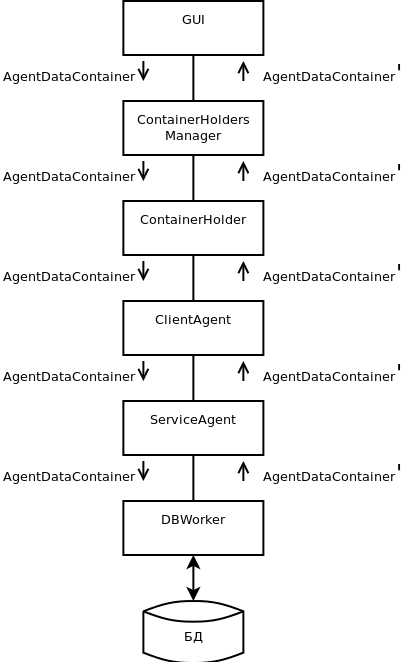
\includegraphics[width=0.5\linewidth]{comm-dia}}
\caption{Коммуникационная модель взаимодействия компонентов системы}
\label{3:comm-dia}
\end{figure}

Содержимое класса состоит из списка массива объектов, хранящих непосредственно табличные данные; массива типа <<Имя-Тип>> для хранения информации о типе и названии колонок данных; а также HashMap'a, содержащего набор <<Ключ-Значение>> для хранения таких параметров как: имя используемой таблицы, строки запроса и т.д.

\paragraph{Класс QueryMaker}
Класс QueryMaker реализует паттерн <<фабрика>> для объектов класса AgentDataContainer.

Основные методы класса:
\begin{itemize}
\item selectTables()~--- производит формирование запроса выборки списка таблиц базы;
\item selectTableContent()~--- производит выборку контента запрашиваемой таблицы;
\item insertData()~--- выполняет добавление строки данных в таблицу;
\item updateData()~--- выполняет модификацию строки данных в таблице.
\end{itemize}

\paragraph{Класс ResponseMaker}
Класс ResponseMaker выполняет сериализацию возвращаемого результа запроса к базе данных. Основной (и единственный) метод класса~--- makeResponse(). Результатом его работы является сформированный объект класса AgentDataContainer, хранящий данные, метадату и дополнительные параметры ответа: имя таблицы и хэш-код ее метадыты.
\begin{lstlisting}
public static AgentDataContainer makeResponse(ResultSet resultSet, AgentDataContainer agentDataContainer) {
    NameTypePair[] metadata = null;
    List<Object[]> data = null;
    String metadataHash = "";

    if (resultSet != null) {
        try {
            ResultSetMetaData rsmd = resultSet.getMetaData();
            int columnCount = rsmd.getColumnCount();
            MetadataHasher.reset();

            metadata = new NameTypePair[columnCount];
            for (int columnIndex = 1; columnIndex <= columnCount; columnIndex++) {
                metadata[columnIndex - 1] = new NameTypePair();
                String name = rsmd.getColumnName(columnIndex);
                int type = rsmd.getColumnType(columnIndex);
                metadata[columnIndex - 1].setName(name);
                metadata[columnIndex - 1].setType(type);

                MetadataHasher.add(type, name);
            }
            metadataHash = MetadataHasher.get();

            data = new ArrayList<Object[]>();
            while (resultSet.next()) {
                Object[] row = new Object[columnCount];
                for (int columnIndex = 1; columnIndex <= columnCount; columnIndex++) {
                    row[columnIndex - 1] = resultSet.getObject(columnIndex);
                }
                data.add(row);
            }
        } catch (SQLException e) {
            e.printStackTrace();
        }
    }

    String tableName = agentDataContainer.getParam(KEY_TABLE_NAME);
    agentDataContainer = new AgentDataContainer(metadata,data);
    agentDataContainer.setParam(KEY_TABLE_NAME, tableName);
    agentDataContainer.setParam(KEY_METADATA_HASH, metadataHash);

    return agentDataContainer;
}
\end{lstlisting}

\subsubsection{Пакет gui}
Набор классов данного пакета реализует графический пользовательский интерфейс приложения. Для егого используется библиотека Swing. Swing относится к библиотеке классов, которая представляет собой набор библиотек для разработки графических оболочек.

Данный пакет включает в себя следующие классы:
\begin{itemize}
\item ClientMainFrame~--- главное окно приложения;
\item ClientTable~--- табличный компонент для отображения данных;
\item ContainerHoldersList~--- список, отображающий доступные контейнеры платформы;
\item InsertDialog~--- модальное окно, осуществляющее добавление данных в таблицу.
\end{itemize}

\paragraph{Класс ClientMainFrame}
Как уже упоминалось выше~--- класс ClientMainFrame реализует главное окно приложения.

Конструктор класса содержит вызов метода initGui(), в котором находятся команды, создающие элементы пользовательского интерфейса: их свойства, параметраы и расположение. После этого производится добавление объекта класса в список подписчиков класса ContainerHoldersManager с его последующим инициализированием.
\begin{lstlisting}
public ClientMainFrame() {
    initGui();

    ContainerHoldersManager.addListener(this);
    ContainerHoldersManager.init();
}
\end{lstlisting}

Основные графические компоненты главного окна:
\begin{itemize}
\item ClientTable table~--- таблица для отображения контента таблиц баз данных;
\item ContainerHoldersList~--- компонент для отображения списка доступных контейнеров;
\item JButton back~--- кнопка для перемещения назад по уровню просматриваемого контента (перемещает к списку таблиц базы из списка записей таблицы);
\item JButton insert~--- кнопка для отображения модального окна добавления строки в таблицу;
\item JPanel bottomBar~--- панель для отображения кнопок back, insert.
\end{itemize}

Расположение элементов осуществляется с помощью механизма <<ограничений>>, накладываемых на каждый компонент. Рассмотрим это на примере компонента ClientTable:
\begin{lstlisting}
GridBagConstraints c = new GridBagConstraints();
...
c.fill = GridBagConstraints.BOTH;
c.weightx = 4.0;
c.weighty = 1.0;
c.gridy = 0;
add(new JScrollPane(table), c);
\end{lstlisting}
Здесь в первой строке происходит создание нового объекта класса <<ограничений>> GridBagConstraints. Далее происходит установка параметров <<растягивания>> компонентов. Константа BOTH указывает компоненту занимать родительское пространство по вертикали и горизонтали. Помимо этого, доступны значения: HORIZONTAL и VERTICAL. Поля weightx и weighty отвечают за <<вес>> компонента по горизонтали и вертикали. <<Вес>> компонента определяет долю занимаемого пространства среди других элементов графического интерфейса, принадлежащих одному родительскому классу. Параметр gridy (и аналогичный ему gridx) определяет положение элемента по высоте (этаж) среди других элементов одного родителя. В последней строке происходит добавление компонента таблицы в состав главного окна приложения, предварительно помещенного в элемент вертикальной прокрутки.

Класс реализует несколько интерфейсов: CHMListener, TableModelListener, ListSelectionListener, ActionListener. Все они служат для обработки событий, поступающих от графических компонентов, а также от класса ControllerHoldersManager для обработки событий, возникающих в ядре системы.

{Пакет utils}
Данный пакет содержит вспомогательные классы и интерфейсы.
\begin{itemize}
\item PrefixGenerator~--- класс служит для генерации уникальных имен для динамически создаваемых агентов;
\item ConditionalVariable~--- мьютекс для ожидания инициализации агента внешним приложением;
\item MatadataHasher~--- класс для создания хэшей стуркур заголовков таблиц;
\item NameTypePair~--- класс, который используется для хранения метадаты таблиц;
\item StringPair~--- вспомогательный класс, используемый для хранения промежуточных данных при генерации параметров для запроса к базе данных;
\item CHMListener~--- интерфейс, реализующий паттерн <<наблюдатель>> для класса ContainerHoldersManager;
\item AgentInterface, AgentData, AgentEvents~--- интерфейсы, реализующие паттерн <<наблюдатель>> для класса Agent.
\end{itemize}

На рисунках ref{3:class-dia1} и ref{3:class-dia2} представлена диаграмма классов проекта. Для лучшей наглядности диаграммы часть классов пакета utils не была представлена ввиду их незначительной функциональной нагрузки.

\begin{figure}[h]
\center{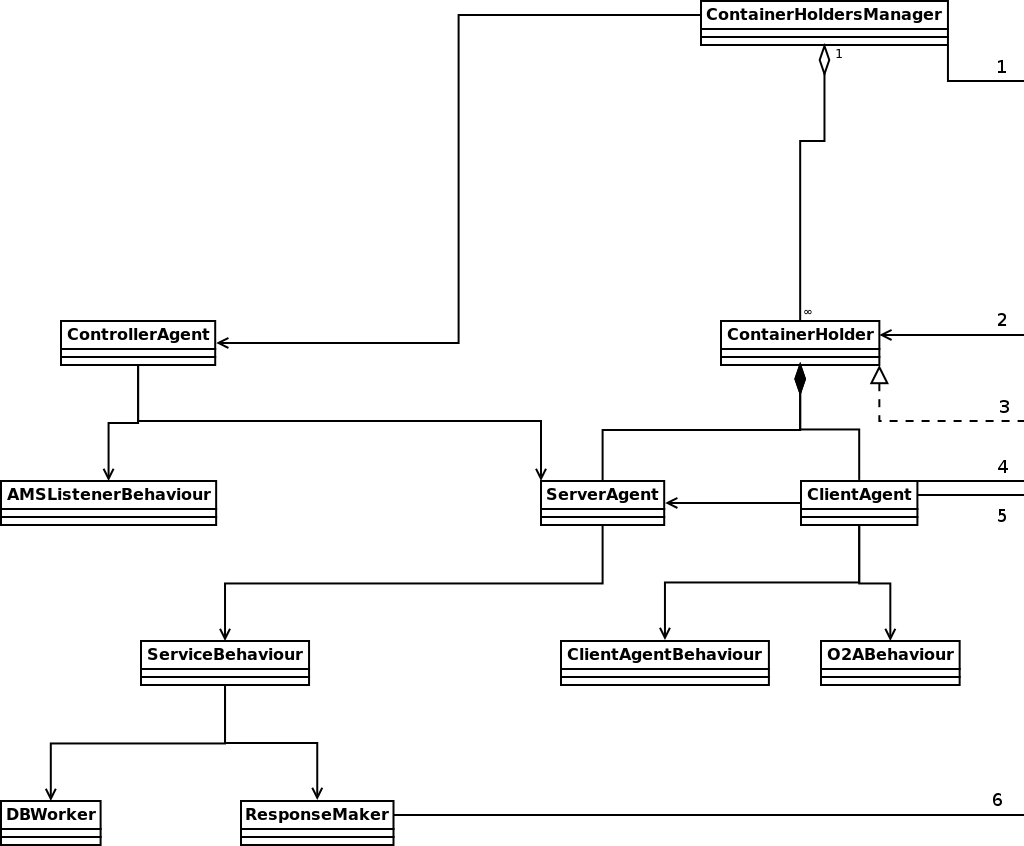
\includegraphics[width=1\linewidth]{class-dia1}}
\caption{Диаграмма классов проекта (начало)}
\label{3:class-dia1}
\end{figure}

\begin{figure}[h]
\center{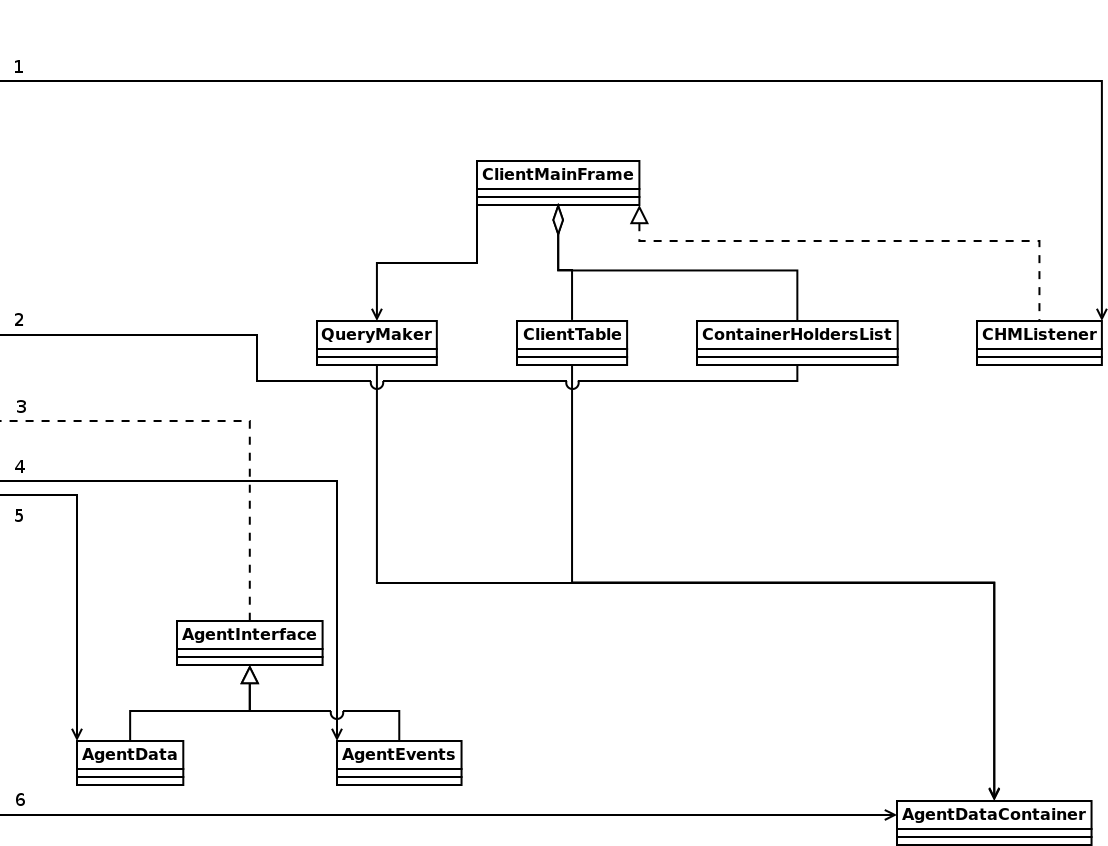
\includegraphics[width=1\linewidth]{class-dia2}}
\caption{Диаграмма классов проекта (окончание)}
\label{3:class-dia2}
\end{figure}

\subsection{Сборка, развертывание и запуск проекта}
Сборка - описать: куда что положить, что запустить.
Развертывание - описать: что сделать на главной машине, что сделать на узлах: поднять postgres и тд.
Запуск - запуск.

\subsubsection{Сборка и развертывание приложения на пользовательском (основном) компьютере}
Для генерации jar файла проекта необходимо запустить в корне проекта команду "mvn package". 
Перед запуском любого приложения, использующего в своем составе jade-агенты, необходимо запустить платформу JADE. Для этого необходимо набрать в командной строке следующую команду:
\begin{lstlisting}
java -cp ~/Downloads/jade.jar jade.Boot -gui
\end{lstlisting}
Это запускает платформу вместе с графическим интерфейсом администрирования (рисунок~ref{3:jade-admin}).
\begin{figure}[h]
\center{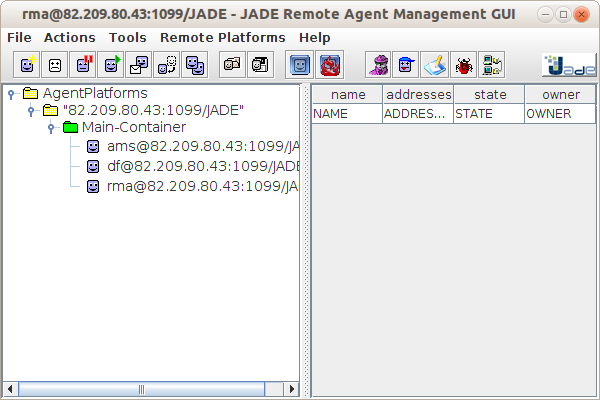
\includegraphics[width=0.7\linewidth]{jade-admin}}
\caption{Панель администрирования платформы JADE}
\label{3:jade-admin}
\end{figure}

Далее запускаем проект в виртуальной машине Java:
\begin{lstlisting}
java -cp target/diploma-1.0-SNAPSHOT-jar-with-dependencies.jar \
    -Dswing.defaultlaf=javax.swing.plaf.nimbus.NimbusLookAndFeel \
        scit.diploma.gui.ClientMainFrame
\end{lstlisting}

\subsubsection{Подготовка и подключение контейнеров на удаленных узлах}
Благодаря технологии мобильных агентов необходимость в установке и настройке <<серверной>> части разрабатываемого проекта отсутствует, однако, существует необходимость некоторой настройки системного окружения и внешних используемых сервисов и приложений на удаленных узлах.
\begin{enumerate}
\item установить и настроить сервер postgresql: приложение использует следующие настройки базы данных:
    \begin{itemize}
        \item имя базы: "postgres";
        \item имя пользователя: "postgres";
        \item пароль: "postgres".
    \end{itemize}
\item запустить платформу JADE следующей командой:
    \begin{lstlisting}
    jade java -cp ~/Downloads/jade.jar jade.Boot -host <hostname> -container <name>
    \end{lstlisting}
\end{enumerate}
Где:
\begin{itemize}
    \item <<hostname>>~--- это IP-адрес платформы основого пользовательного приложения системы;
    \item <<name>>~--- имя создаваемого контейнера;
\end{itemize}
На этом процесс настройки удаленного узла закончен. После создания контейнера на удаленной машине, он будет мгновенно отображен в списке доступных контейнеров в интерфейсе главного пользовательского приложения.

\subsection{Использование приложения}
После запуска программы на пользовательском компьютере окрывается главное окно, разделенное на три логических части (рисунок~\ref{3:proga}):
\begin{itemize}
\item список доступных и активных контейнеров~--- слева;
\item основной информационный контент~--- справа;
\item дополнительная панель~--- находящаяся под списком контейнеров.
\end{itemize}

\begin{figure}[h!]
\center{\includegraphics[width=1\linewidth]{proga}}
\caption{Главное окно программы}
\label{3:proga}
\end{figure}

В это время система подписывается на события регистрации новых контейнеров в составе платформы JADE. При добавлении нового контейнера в платформу~--- он будет мгновенно отображен в списке доступных контейнеров.

При клике по контейнеру происходит его активация. После процесса активации автоматически происходит запрос у сервера базы данных контейнера списка имеющихся таблиц.

Клик по выбранной сроке в списке таблиц отправляет запрос сервису на получение контента выбранной таблицы. После ответа сервиса на панели справа отображаются данные этой таблицы. Следует отметить, что первой колонкой в отображаемом контенте помещается имя контейнера, с которого получены данные.

\begin{figure}[h!]
\center{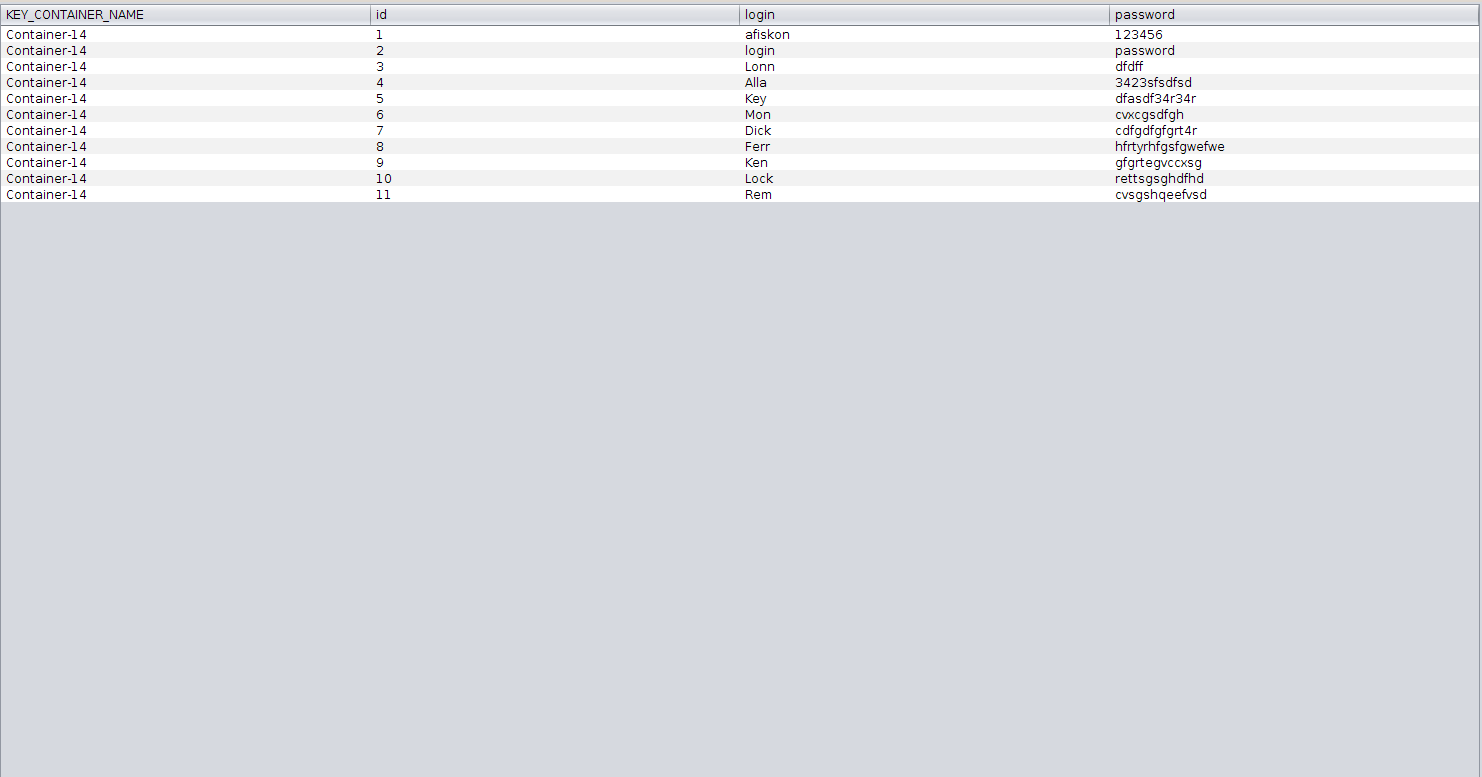
\includegraphics[width=1\linewidth]{content}}
\caption{Контент запрашиваемой таблицы}
\label{3:content}
\end{figure}

Двойной клик на выбранной строке таблицы переводит пользователя в режим редактирования данных. Ввод нового значения в ячейку таблицы сопровождается отправкой соотвествующему сервису данных модифицированной строки на перезапись в базу.

\begin{figure}[h!]
\center{\includegraphics[width=1\linewidth]{update}}
\caption{Процесс редактирования таблицы}
\label{3:update}
\end{figure}

Для добавления данных в таблицу необходимо нажать кнопку <<Вставить>>, расположенную на панели внизу. Здесь возможны два варианта: простое добавление данных в текущую таблицу кнопкой <<Вставить>>, либо добавление данных с реплицированием на другие узлы кнопкой <<Вставить с реплицированием>>.

\begin{figure}[h!]
\center{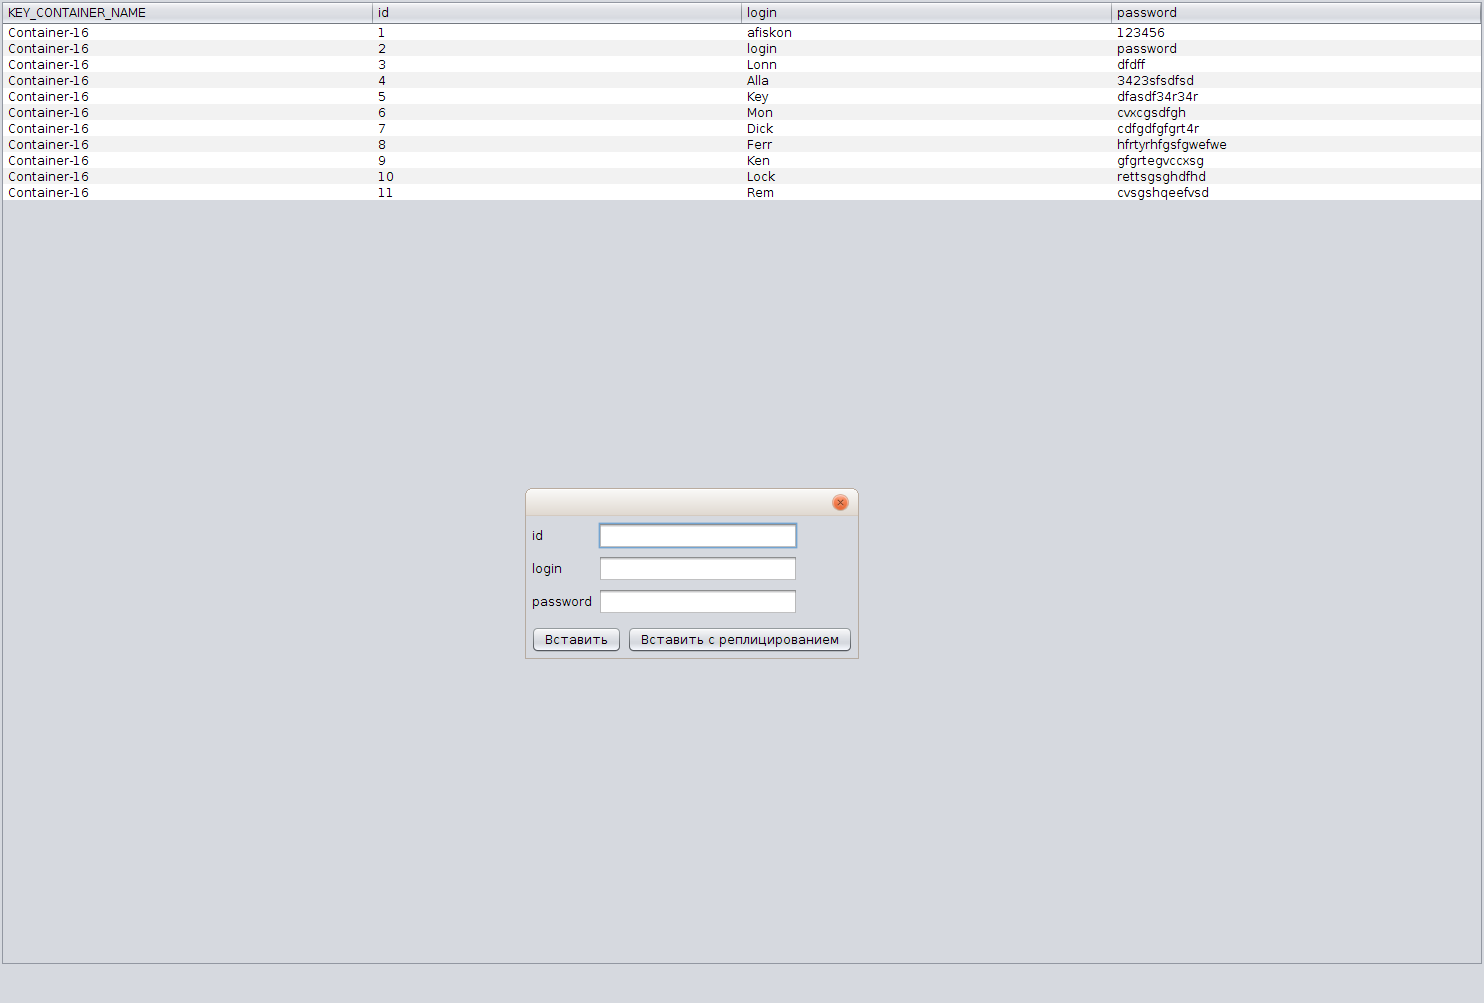
\includegraphics[width=1\linewidth]{insert}}
\caption{Добавление данных в таблицу}
\label{3:insert}
\end{figure}

Для выполнения пользовательского rawsql-запроса следует нажать кнопку <<Raw-запрос>>. При этого появится аналогичное окно с возможностью простого запроса и запроса с репликацией.

\begin{figure}[h!]
\center{\includegraphics[width=1\linewidth]{raw}}
\caption{Диалоговое окно выполнения rawsql-запросов}
\label{3:raw}
\end{figure}

Кнопка <<Назад>> выполняет переход на список таблиц контейнера из режима отображения контента таблицы.

На рисунке~\ref{3:usecase} приведена диаграмма вариантов использования приложения.
\begin{figure}[h!]
\center{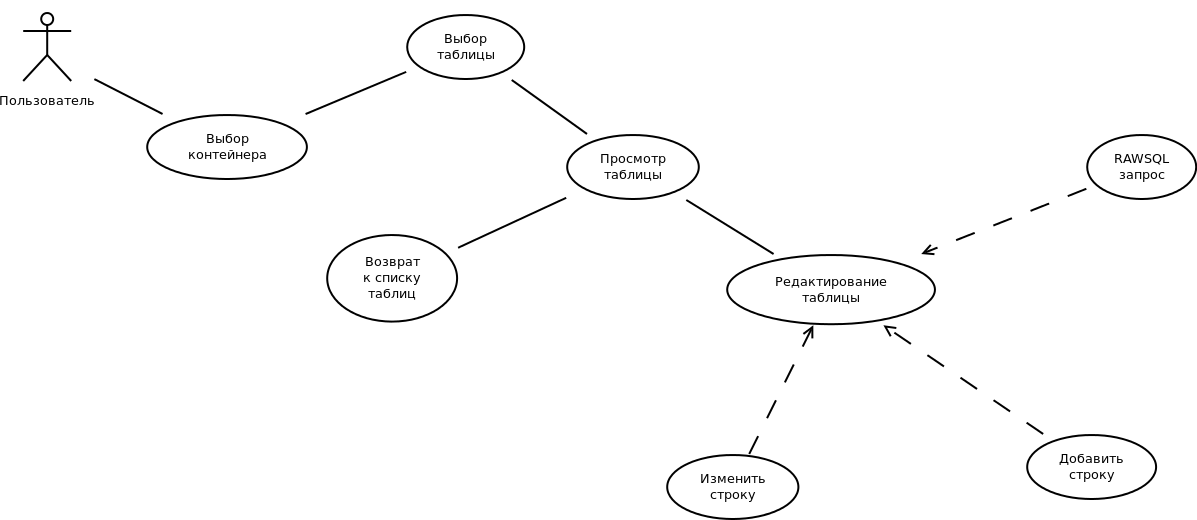
\includegraphics[width=1\linewidth]{usecase}}
\caption{Диаграмма вариантов использования приложения}
\label{3:usecase}
\end{figure}
